%=================
\chapter{Sprint I}
%=================

\section{Sprint planning}
%------------------------
In our first sprint we will implement basic and fundamental parts of the utility. Based on the pre-study, we have decided what preprocessor and parser to use, so the task is to make this work together and achieve the desired functionality.  

\subsection{Duration}
%-----------------
Sprint 1 started September 14th, and lasted until September 27th. To ensure an understanding between our developers and the customer, we will have weekly meetings to show what we have accomplished and discuss further development. 

\subsection{Sprint goal}
%--------------------
The overall goal of the sprint 1 is to create a preliminary design and implement the core of the application. It will be possible to run it and generate the Lua script and therefore it can be used by Wireshark users. The first version will contain only the basic dissector generating features, i.e. parsing simple data structures. Also, some of the preprocessing capabilities will be implemented, such as handling \#include directives. Basic support for configuration will be added.

\subsection{Back log}
%-----------------
The first sprint we will implement eight requirements. Table \ref{tab:sp1_req7a}-\ref{tab:sp1_req2d}  list each requirement with a time estimate.\\
\autoref{tab:sprint1req} is the sprint backlog for the first phase. \\
\autoref{tab:sprint1time} is the time table for the first phase. \\
\begin{table}[!ht] \small \center
\caption{Sprint 1 Requirement FR7-A} \label{tab:sp1_req7a}
\begin{tabular}{l l c}
	\toprule
	Requirement & Task & Hours \\
	\midrule
	\multirow{4}{5cm}{Command line shall support parameters for c-header file} & Design & 1 \\
	& Implementation & 2 \\
	& Testing & 2 \\
	& Documentation & 4 \\
	\bottomrule
\end{tabular}
\end{table}

\begin{table}[!ht] \small \center
\caption{Sprint 1 Requirement FR1-A} \label{tab:sp1_req1a}
\begin{tabular}{l l c}
	\toprule
	Requirement & Task & Hours \\
	\midrule
	\multirow{4}{5cm}{The utility must support the following basic data types: int, float, char and boolean} & Design & 4 \\
	& Implementation & 8 \\
	& Testing & 8 \\
	& Documentation & 4 \\
	\bottomrule
\end{tabular}
\end{table}

\begin{table}[!ht] \small \center
\caption{Sprint 1 Requirement FR2-A} \label{tab:sp1_req2a}
\begin{tabular}{l l c}
	\toprule
	Requirement & Task & Hours \\
	\midrule
	\multirow{4}{5cm}{The dissector shall be able to display simple structs} & Design & 4 \\
	& Implementation & 8 \\
	& Testing & 8 \\
	& Documentation & 8 \\
	\bottomrule
\end{tabular}
\end{table}

\begin{table}[!ht] \small \center
\caption{Sprint 1 Requirement FR3-A} \label{tab:sp1_req3a}
\begin{tabular}{l l c}
	\toprule
	Requirement & Task & Hours \\
	\midrule
	\multirow{4}{5cm}{The utility shall support \#include} & Design & 2 \\
	& Implementation & 2 \\
	& Testing & 2 \\
	& Documentation & 2 \\
	\bottomrule
\end{tabular}
\end{table}

\begin{table}[!ht] \small \center
\caption{Sprint 1 Requirement FR3-B} \label{tab:sp1_req3b}
\begin{tabular}{l l c}
	\toprule
	Requirement & Task & Hours \\
	\midrule
	\multirow{4}{5cm}{The utility shall support \#define and \#if} & Design & 1 \\
	& Implementation & 2 \\
	& Testing & 6 \\
	& Documentation & 2 \\
	\bottomrule
\end{tabular}
\end{table}

\begin{table}[!ht] \small \center
\caption{Sprint 1 Requirement FR7-B} \label{tab:sp1_req7b}
\begin{tabular}{l l c}
	\toprule
	Requirement & Task & Hours \\
	\midrule
	\multirow{4}{5cm}{Command line shall support for configuration file} & Design & 8 \\
	& Implementation & 8 \\
	& Testing & 8 \\
	& Documentation & 4 \\
	\bottomrule
\end{tabular}
\end{table}

\begin{table}[!ht] \small \center
\caption{Sprint 1 Requirement FR4-A}\label{tab:sp1_req4a}
\begin{tabular}{l l c}
	\toprule
	Requirement & Task & Hours \\
	\midrule
	\multirow{4}{5cm}{Configuration must support valid ranges for struct members} & Design & 6 \\
	& Implementation & 8 \\
	& Testing & 8 \\
	& Documentation & 8 \\
	\bottomrule
\end{tabular}
\end{table}

\begin{table}[!ht] \small \center
\caption{Sprint 1 Requirement FR2-D} \label{tab:sp1_req2d}
\begin{tabular}{l l c}
	\toprule
	Requirement & Task & Hours \\
	\midrule
	\multirow{4}{5cm}{The dissector shall be able to recognize invalid values for a struct member} & Design & 4 \\
	& Implementation & 6 \\
	& Testing & 8 \\
	& Documentation & 4 \\
	\bottomrule
\end{tabular}
\end{table}

\begin{table}[!ht] \small \center
\caption{Sprint 1 Requirements \label{tab:sprint1req}}
\begin{tabularx}{\textwidth}{l l X c c}
	\toprule
	& & & \multicolumn{2}{c}{Hours} \\
	\cmidrule(r){4-5}
	\# & Req. & Description & Est. & Act. \\
	\midrule
	1 & FR7-A & Command line shall support parameters for c-header file & 9 & 6\\
	\addlinespace
	2 & FR1-A & Support basic data types: int, float, char, boolean & 24 & 20\\
	\addlinespace
	3 & FR2-A & The dissector shall be able to display simple structs & 28 & 25\\
	\addlinespace
	4 & FR3-A & The utility shall support \#include & 8 & 2\\
	\addlinespace
	5 & FR3-B & The utility shall support \#define and \#if & 11 & 3\\	
	\addlinespace
	6 & FR7-B & Command line shall support for configuration file & 28 & 8\\
	\addlinespace
	7 & FR4-A & Support valid ranges for struct members & 30 & 15 \\
	\addlinespace
	8 & FR2-D & Recognize invalid values for a struct member & 22 & 12\\
	\midrule
	& & Total: & 160 & 91\\
	\bottomrule
\end{tabularx}
\end{table}

\begin{table}[!ht] \small \center
\caption{Sprint 1 Timetable\label{tab:sprint1time}}
\begin{tabularx}{\textwidth}{X c c}
	\toprule
	& \multicolumn{2}{c}{Hours} \\
	\cmidrule(r){2-3}
	Description & Est. & Act. \\
	\midrule
	Design & 30 & 10\\
	\addlinespace
	Implementation & 44 & 65 \\
	\addlinespace
	Testing & 50 & 15\\
	\addlinespace
	Documentation & 36 & 1\\
	\midrule
	Total: & 160 & 91\\
	\bottomrule
\end{tabularx}
\end{table} 

\section{Sprint Design}
This section introduces the design of the system modules implemented in sprint 1

\subsection{Utility}
Figure \ref{fig:sp1_class} illustrates the current class diagram for this sprint 1. The CSjark module contains the main method of the utility and is responsible for running the program. The utility will typically start off by using cparser to parse the c-header file given to the utility as a command line argument. Cparser will then use the config module to ensure that the parsing is done correctly after the configuration, and then generate protocols and fields to be used in the CSjark module. The CSjark module then generates a wireshark dissector in LUA code by going through the protocols and fields generated earlier by the cparser module. 

\begin{figure}[!ht]
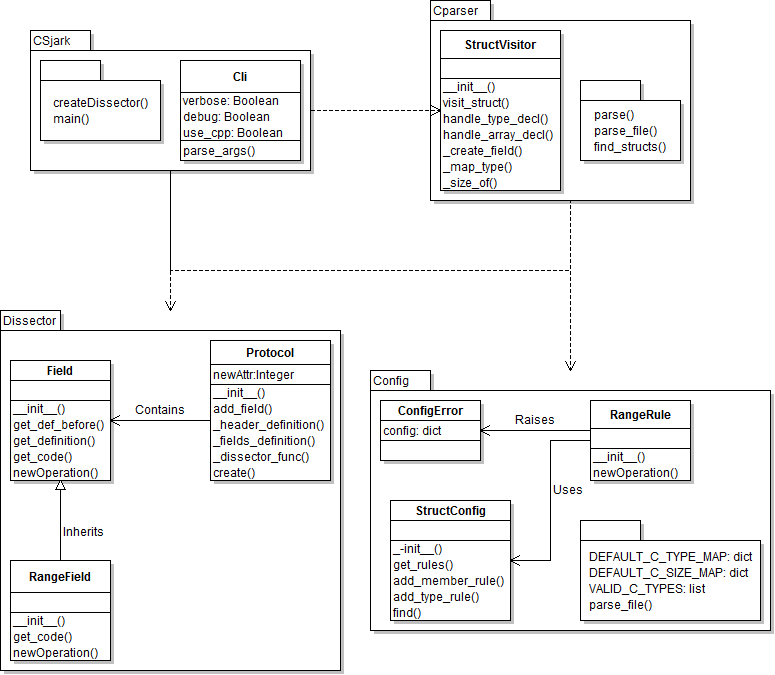
\includegraphics[width=\textwidth]{./sprints/img/class_diagram_s1.png}
\caption{Class Diagram}
\label{fig:sp1_class}
\end{figure}

\section{Implementation}

In this sprint we have created a very naive implementation of the utility. It supports the most basic types of C-structs. In addition the utility supports some basic configuration.

We have decided to use YAML as our configuration format. In this sprint we have added support for range specification.
A user can specify the ranges of the members of a struct, from a minimum to a maximum.
In figure \ref{fig:dissector_screenshot} below you can see how Wireshark displays a member that has an invalid range. \newline
\begin{figure}[!ht]
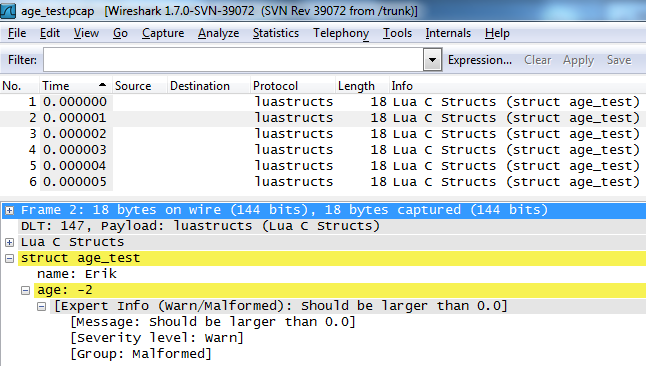
\includegraphics[width=\textwidth]{./sprints/img/wireshark_outofrange.png}
\caption{Wireshark dissector}
\label{fig:dissector_screenshot}
\end{figure}	

The tool uses a command line interface. The user inputs a header-file and optionally a configuration file to the command line, and the program outputs a Lua-script.  Below you can see a figure \ref{fig:cmd_screenshot} that illustrates how the program is run.
\begin{figure}[!ht]
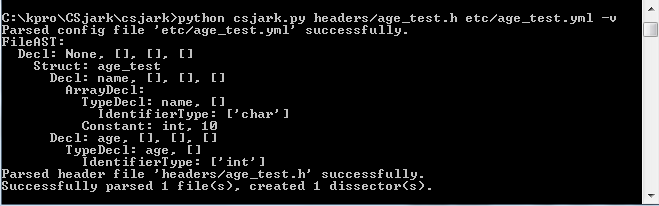
\includegraphics[width=\textwidth]{./sprints/img/cmd_agetest_run.png}
\caption{Command line}
\label{fig:cmd_screenshot}
\end{figure}

\section{Sprint Testing}
This section introduces the tests preformed during the sprint and their results

\subsection{Tests}
During the sprint the team executed a total of 7 tests with names as seen below\\

\noindent Tests executed:

\begin{itemize}
\item TID01 - Supporting parameters for c-header file\autoref{tab:TID1}
\item TID02 - Supporting basic data types\autoref{tab:TID2}
\item TID03 -  Displaying simple structs \autoref{tab:TID3}
\item TID04 - Supporting c-header files with the \#include directive\autoref{tab:TID4}
\item TID05 - Supporting \#define and \#if\autoref{tab:TID5}
\item TID06 - Supporting configuration files\autoref{tab:TID6}
\item TID07 - Recognizing invalid values\autoref{tab:TID7}
\end{itemize}

\subsection{Test Results}
The test results can be seen in table \ref{tab:sp1_tid01}-\ref{tab:sp1_tid07}.
\begin{table}[!ht] \footnotesize \center
\caption{Supporting parameters for c-header file \label{tab:sp1_tid01}}
\noindent\makebox[\textwidth]{%
\begin{tabularx}{\textwidth}{l X}
	\toprule
	Portion & Description \\
	\midrule
	Description & Supporting parameters for c-header file \\
	Tester & Lars Solvoll Tønder \\
	Date & 27.09.2011 \\
	Result & Failure. The LUA-file got created successfully but the user was not informed of the result \\
	\bottomrule
\end{tabularx}}
\end{table}

\begin{table}[!ht] \footnotesize \center
\caption{Supporting basic data types \label{tab:sp1_tid02}}
\noindent\makebox[\textwidth]{%
\begin{tabularx}{\textwidth}{l X}
	\toprule
	Portion & Description \\
	\midrule
	Description & Supporting basic data types \\
	Tester & Lars Solvoll Tønder \\
	Date & 27.09.2011 \\
	Result & Failure. The program supports the use of int, float, char and boolean, but did not inform the user of the result\\
	\bottomrule
\end{tabularx}}
\end{table}

\begin{table}[!ht] \footnotesize \center
\caption{Displaying simple structs  \label{tab:sp1_tid03}}
\begin{tabular}{l l}
	\toprule
	Portion & Description \\
	\midrule
	Description & Displaying simple structs \\
	Tester & Lars Solvoll Tønder \\
	Date & 27.09.2011 \\
	Result & Failure.Success\\
	\bottomrule
\end{tabular}
\end{table}

\begin{table}[!ht] \footnotesize \center
\caption{Supporting c-header files with the \#include directive \label{tab:sp1_tid04}}
\noindent\makebox[\textwidth]{%
\begin{tabularx}{\textwidth}{l X}
	\toprule
	Portion & Description \\
	\midrule
	Description &  Supporting c-header files with the \#include directive  \\
	Tester & Lars Solvoll Tønder \\
	Date & 27.09.2011 \\
	Result & Failure. The program supports header files with the \#include directive, but did not inform the user of the result\\
	\bottomrule
\end{tabularx}}
\end{table}

\begin{table}[!ht] \footnotesize \center
\caption{Supporting \#define and \#if \label{tab:sp1_tid05}}
\noindent\makebox[\textwidth]{%
\begin{tabularx}{\textwidth}{l X}
	\toprule
	Portion & Description \\
	\midrule
	Description &  Supporting \#define and \#if  \\
	Tester & Lars Solvoll Tønder \\
	Date & 27.09.2011 \\
	Result & Failure. The program supports header files with the \#define and \#if directives, but did not inform the user of the result\\
	\bottomrule
\end{tabularx}}
\end{table}

\begin{table}[!ht] \footnotesize \center
\caption{Supporting configuration files \label{tab:sp1_tid06}}
\noindent\makebox[\textwidth]{%
\begin{tabularx}{\textwidth}{l X}
	\toprule
	Portion & Description \\
	\midrule
	Description &  Supporting configuration files  \\
	Tester & Lars Solvoll Tønder \\
	Date & 27.09.2011 \\
	Result & Failure. The program supports the use of configuration files but does not inform the user of any results\\
	\bottomrule
\end{tabularx}}
\end{table}

\begin{table}[!ht] \footnotesize \center
\caption{Recognizing invalid values \label{tab:sp1_tid07}}
\begin{tabular}{l l}
	\toprule
	Portion & Description \\
	\midrule
	Description &  Recognizing invalid values  \\
	Tester & Lars Solvoll Tønder \\
	Date & 27.09.2011 \\
	Result & Success\\
	\bottomrule
\end{tabular}
\end{table}

\subsection{Test Evaluation}
Most of our tests failed because the developers had forgotten to implement usability features presenting the user with any textual information. Even so, with all the core functionality in place it didn't take the developers much time to fix these errors.

\section{Customer Feedback}

\subsection{Pre-sprint}
The customer had no objections to the contents of the first sprint, but was not completely satisfied with the feature descriptions. They thought that we should have much more implementation details for each requirement, and that each requirement should be properly broken down, also in the sense that implementation and design should be two separate tasks if design is necessary. Corollary to this, our work items were too big. They also suggested a proper finish condition for each work item.
\subsection{Post-sprint}
We presented the result from the sprint 1 for the customer and they were very happy with the result. They had some ideas for how we could make our configuration files more compact, but said that this was not really an important thing. Their other comments were mostly around what they wanted us to do for sprint 2 and how those features might be implemented.

\section{Sprint Evaluation}
This section contains the team evaulation of the first sprint.
\subsection{Review}
The first sprint is over and the team has implemented a working utility. During the sprint planning we decided which requirements from the product backlog that we were to fulfill during the first sprint. The product backlog contains a prioritized list of requirements. We decided to include the requirements that had the highest prioritization. These requirements were basic, but essential and therefore high prioritized.
   
The lack of prior knowledge to scrum made planning and execution of the sprint complicated for the team. We did not agree within the team of how to do it, and wasted some time on discussion going back and forth. In the end we understood that we gave a too high level description of the requirements, and had to redo previous work. This was time consuming, stealing person-hours from other parts of the sprint.

Each requirement is divided in four parts: design, implementation, testing and documentation. We currently have most of these parts covered, except documentation for all files and unit test for the dissector file. This work is postponed till the second sprint.

The first sprint resulted in a solid core for our project. The customer was happy with the first demo they got, the utility even run on Mac (which was overwhelming for Stig). We feel that we have a good start and are confident that we will be able to give the customer the product that they want in the end.

The burndown chart shows the progress during the first sprint. The team made an effort in making a correct estimation. This is reflected in the chart, as the estimated and actual hours are  following each other closely. At the end actual hours stops at 11 hours, which means we have some undone tasks. These are put back in the product backlog, and will probably be part of the next sprint. 

\begin{figure}[!ht]
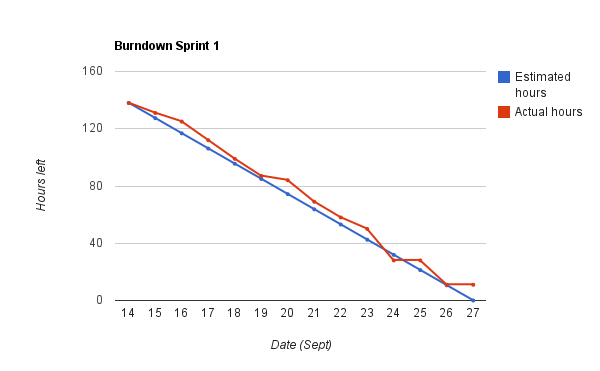
\includegraphics[width=\textwidth]{./sprints/img/burndown_chart_s1.png}
\caption{Burndown chart}
\label{fig:sp1_burndown}
\end{figure}

\subsection{Positive Experiences}
\begin{itemize}
	\item Good customer communication and relation from the beginning
	\item Implementation was easy
	\item Most of the requirements for this sprint were completed
	\begin{itemize} 
		\item all design, implementation and testing were completed
		\item documentation had to be putted back in the product backlog 
	\end{itemize}
	\item Errors and bugs were detected and corrected swiftly and with relative ease
	\item The team functioned well, with sufficient discussions and conflicts
\end{itemize}
\subsection{Negative Experiences}
\begin{itemize}
	\item Hard for the team members to “give” 25 person-hours each week
	\begin{itemize}
		\item to understand that it is needed
		\item to free up so many hours, and still have time to do other subjects
	\end{itemize}
	\item Hard to find time for meeting/work where all team members was able to meet
	\item One member of the team got sick
	\item We did not document the process and work during the first sprint well enough, which was a burden at the end of the sprint
	\item We did perhaps not understand scrum properly, which resulted in extra work
\end{itemize}
\subsection{Planned Actions}
\textbf{Better sprint planning} \newline
In order to avoid having to redo much of the work because of incorrect/poorly sprint planning, we have decided to do this properly next time. We have learned what we need to have in place and how to document it from this sprint. \newline
\textbf{Design early in the sprint} \newline
The design should be in place early in the sprint. This is related to better sprint planning, the planning should be so detailed/good that additional design is not necessary. This is important for understanding and being able to estimate hours and divide work. \newline
\textbf{Documenting in parallel while implementing} \newline
We suffered from the problem code first, then document. This is not a good practise in team divided work. We will try to do the documentation as we code.
The documents for the project report also experienced a standstill while the team worked on implementation. Writing parts of sprint documentation while having the sprint is a much better way to work, then most part of the documentation is already done before the sprint evaluation. \newline
\textbf{Split coding and report writing between team members} \newline
Not all the team members have to do coding. It is important to maintain a steady progress making the project report (which our grade evaluation is based on), while doing the implementation. Responsibilities for coding and report will be assigned next sprint. \newline
\subsection{Barriers}
Some of the team members has experience some technical difficulties with their Git client, and others had problems setting up PyCharm. Problems rose as we realized that there would be hard setting up the programs on different platforms (Windows and Mac).

We had problems with c parser library(pycparser), which did not support \_Bool type, specified in the C99 standard. A patch for this was written by Even, and was later included in the pycparser library. There was also problems with the testing framework(attest), this framework did not have support for Windows command line prompt, a patch was written and was later added to their library.

Some team members had conflicting deadlines for deliveries in different courses.  